\chapter{Apéndice}\label{chapter:apendice}

A continuación se presentan algunos ejemplos de subtítulos generados.

\begin{figure}[h!]
    \centering
    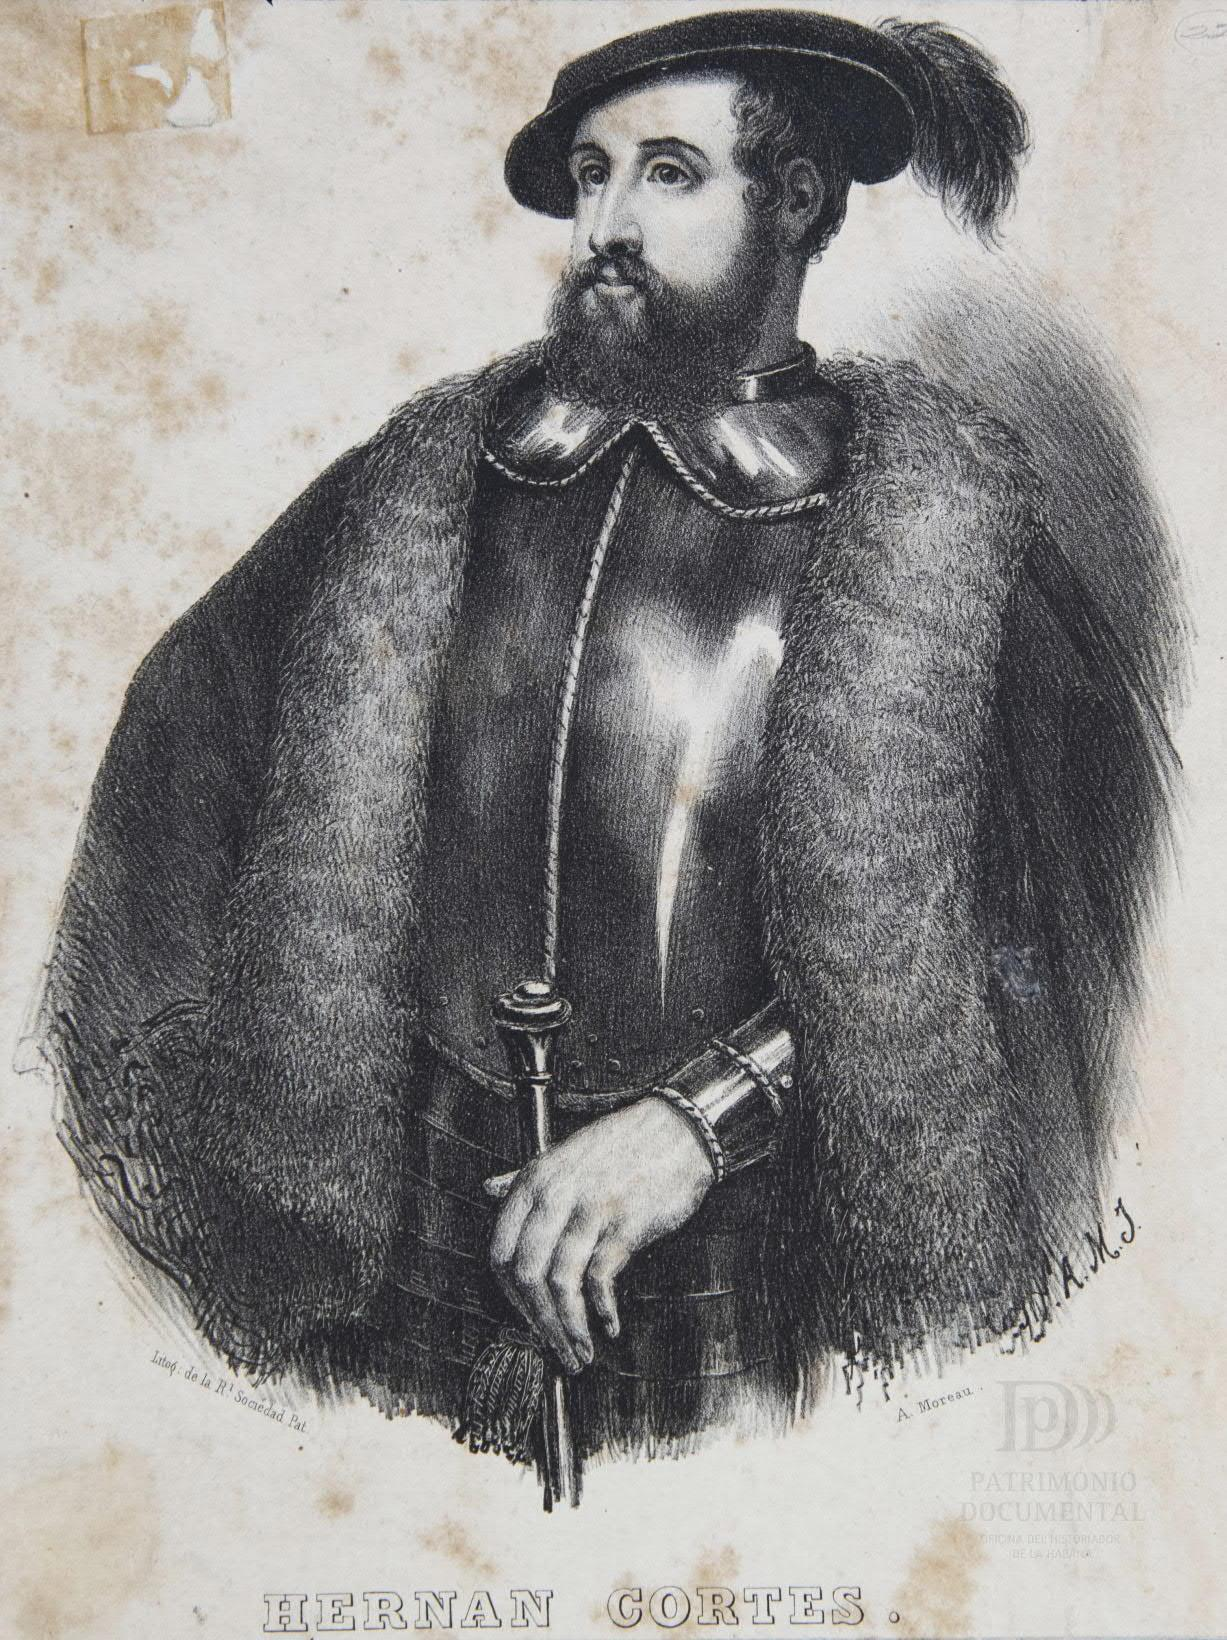
\includegraphics[width=0.5\textwidth]{Graphics/un dibujo de un hombre con un abrigo de piel.jpg}
    \caption{Un dibujo de un hombre con un abrigo de piel (Exitoso)}
\end{figure} 
\begin{figure}[h!]
    \centering
    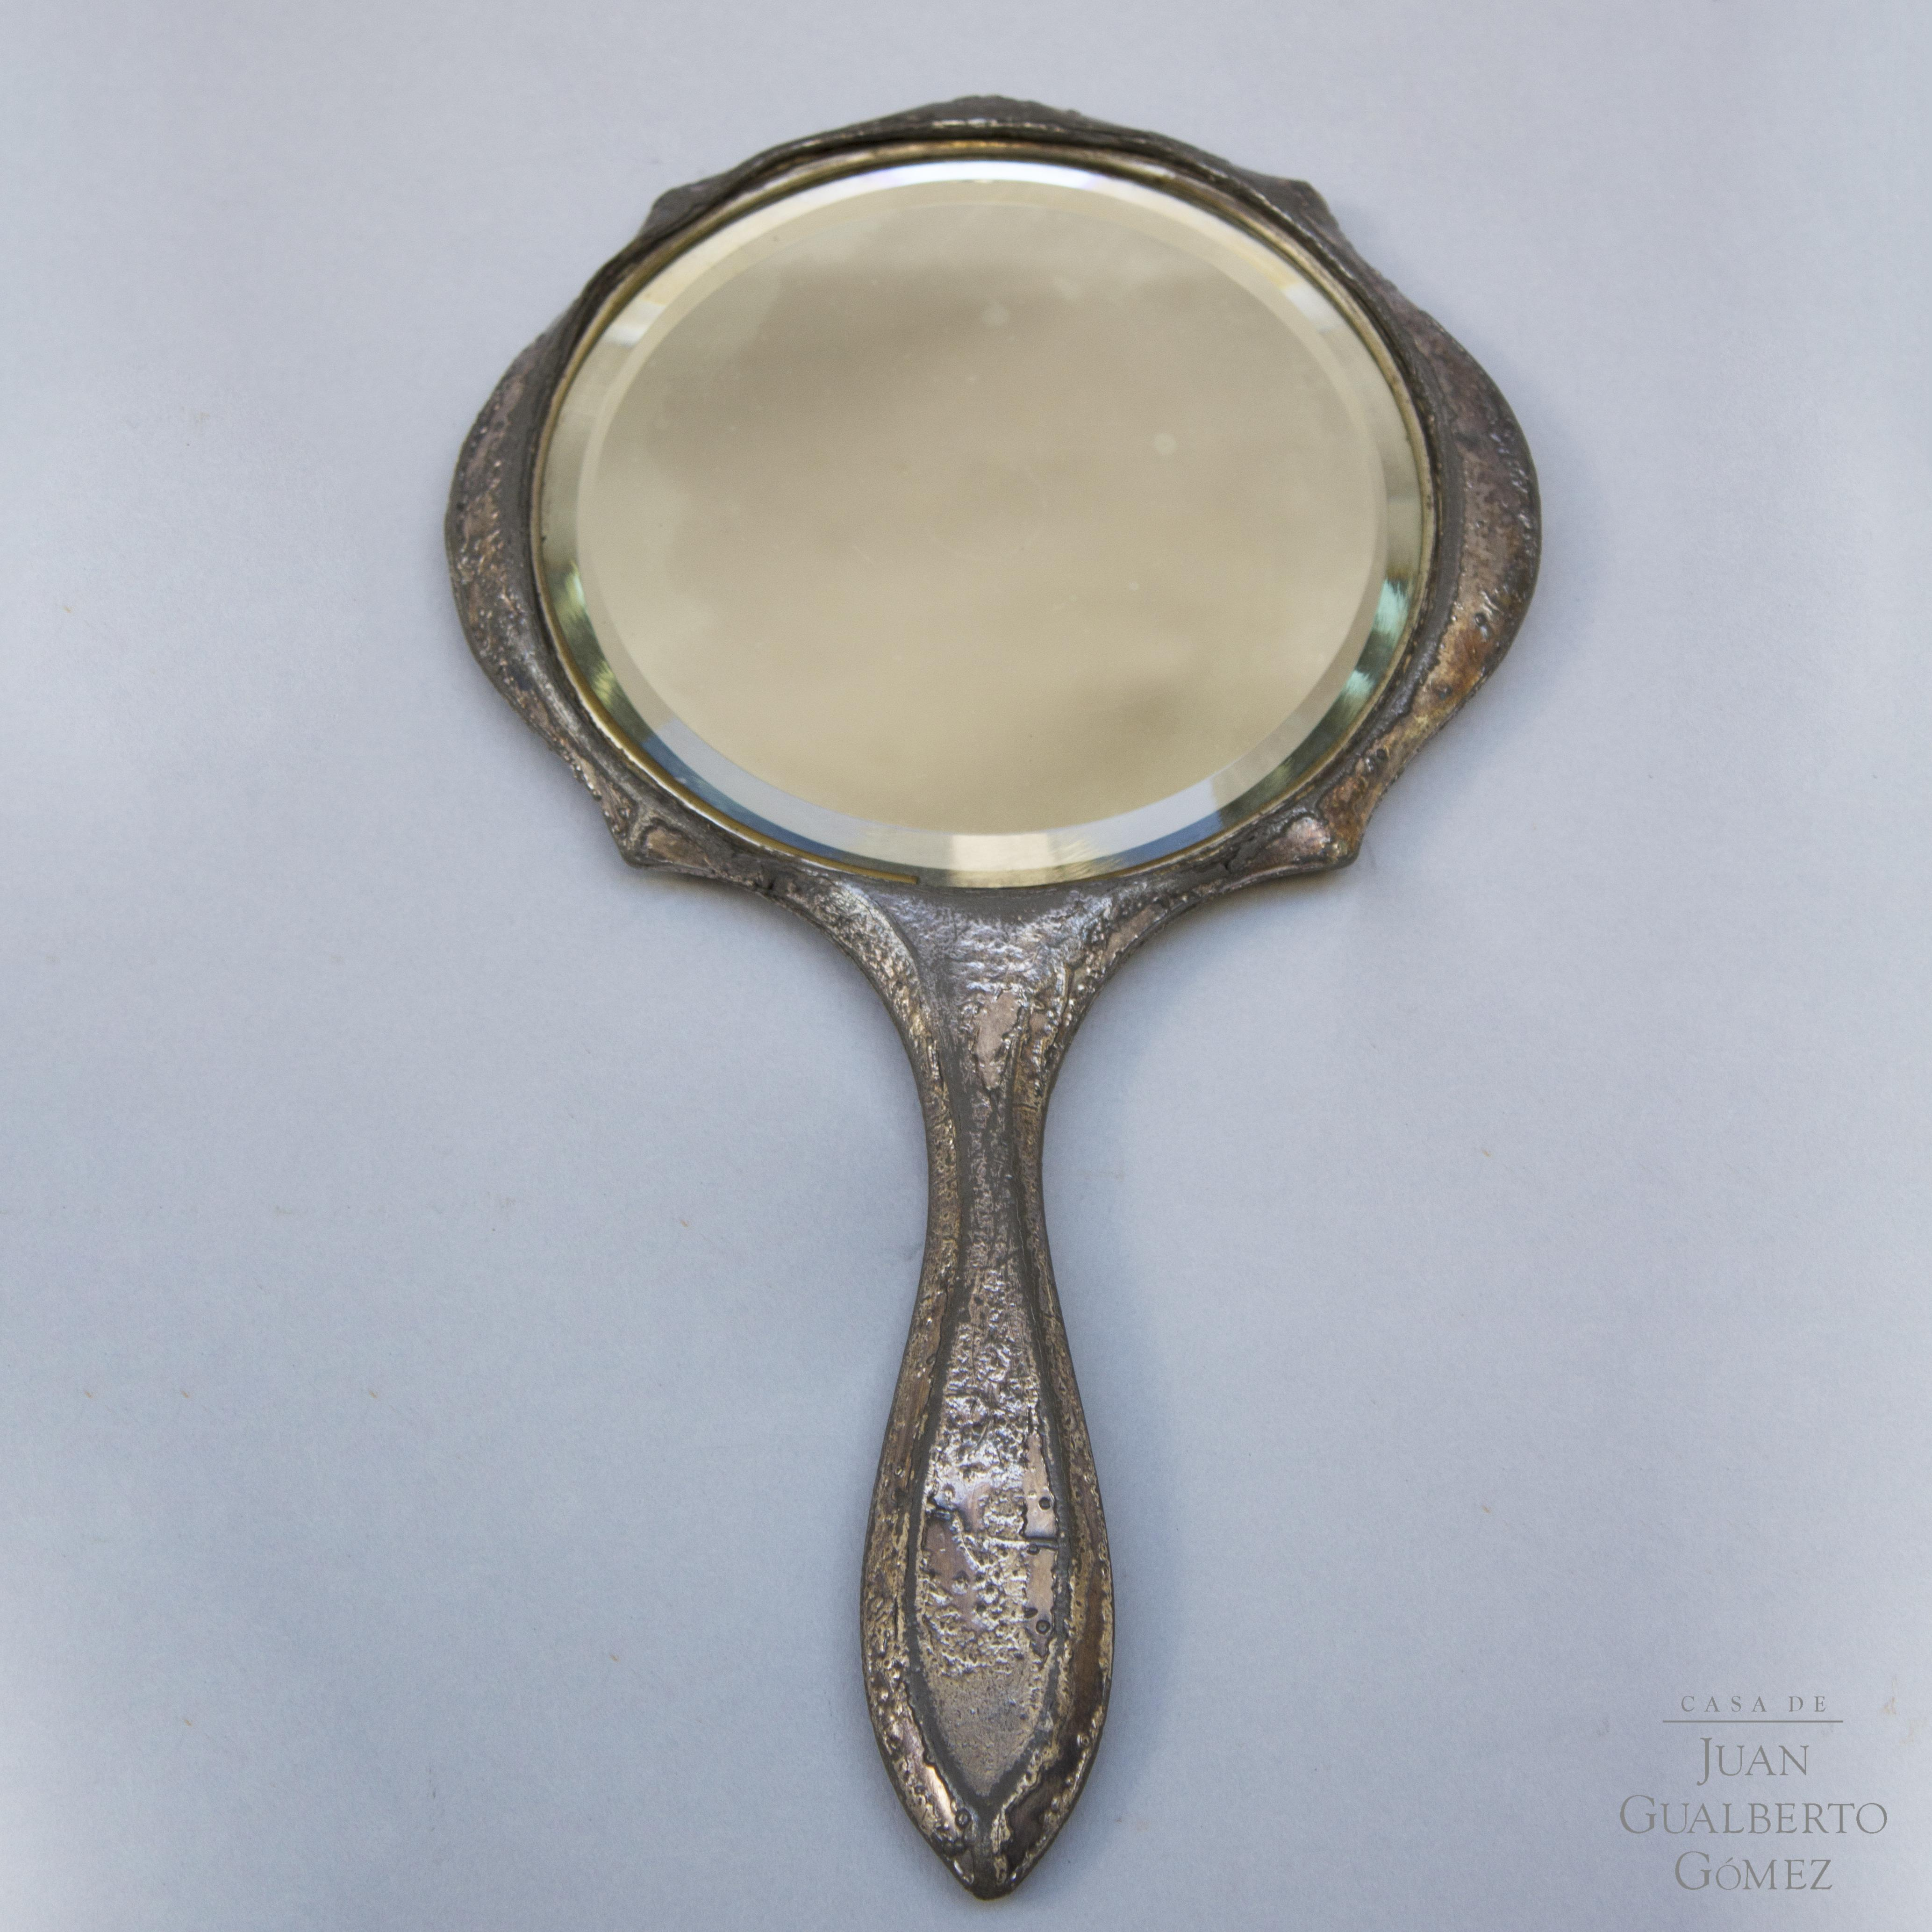
\includegraphics[width=0.5\textwidth]{Graphics/un espejo con un mango de plata.jpg}
    \caption{Un espejo con un mango de plata (Exitoso)}
\end{figure}
\begin{figure}[h!]
    \centering
    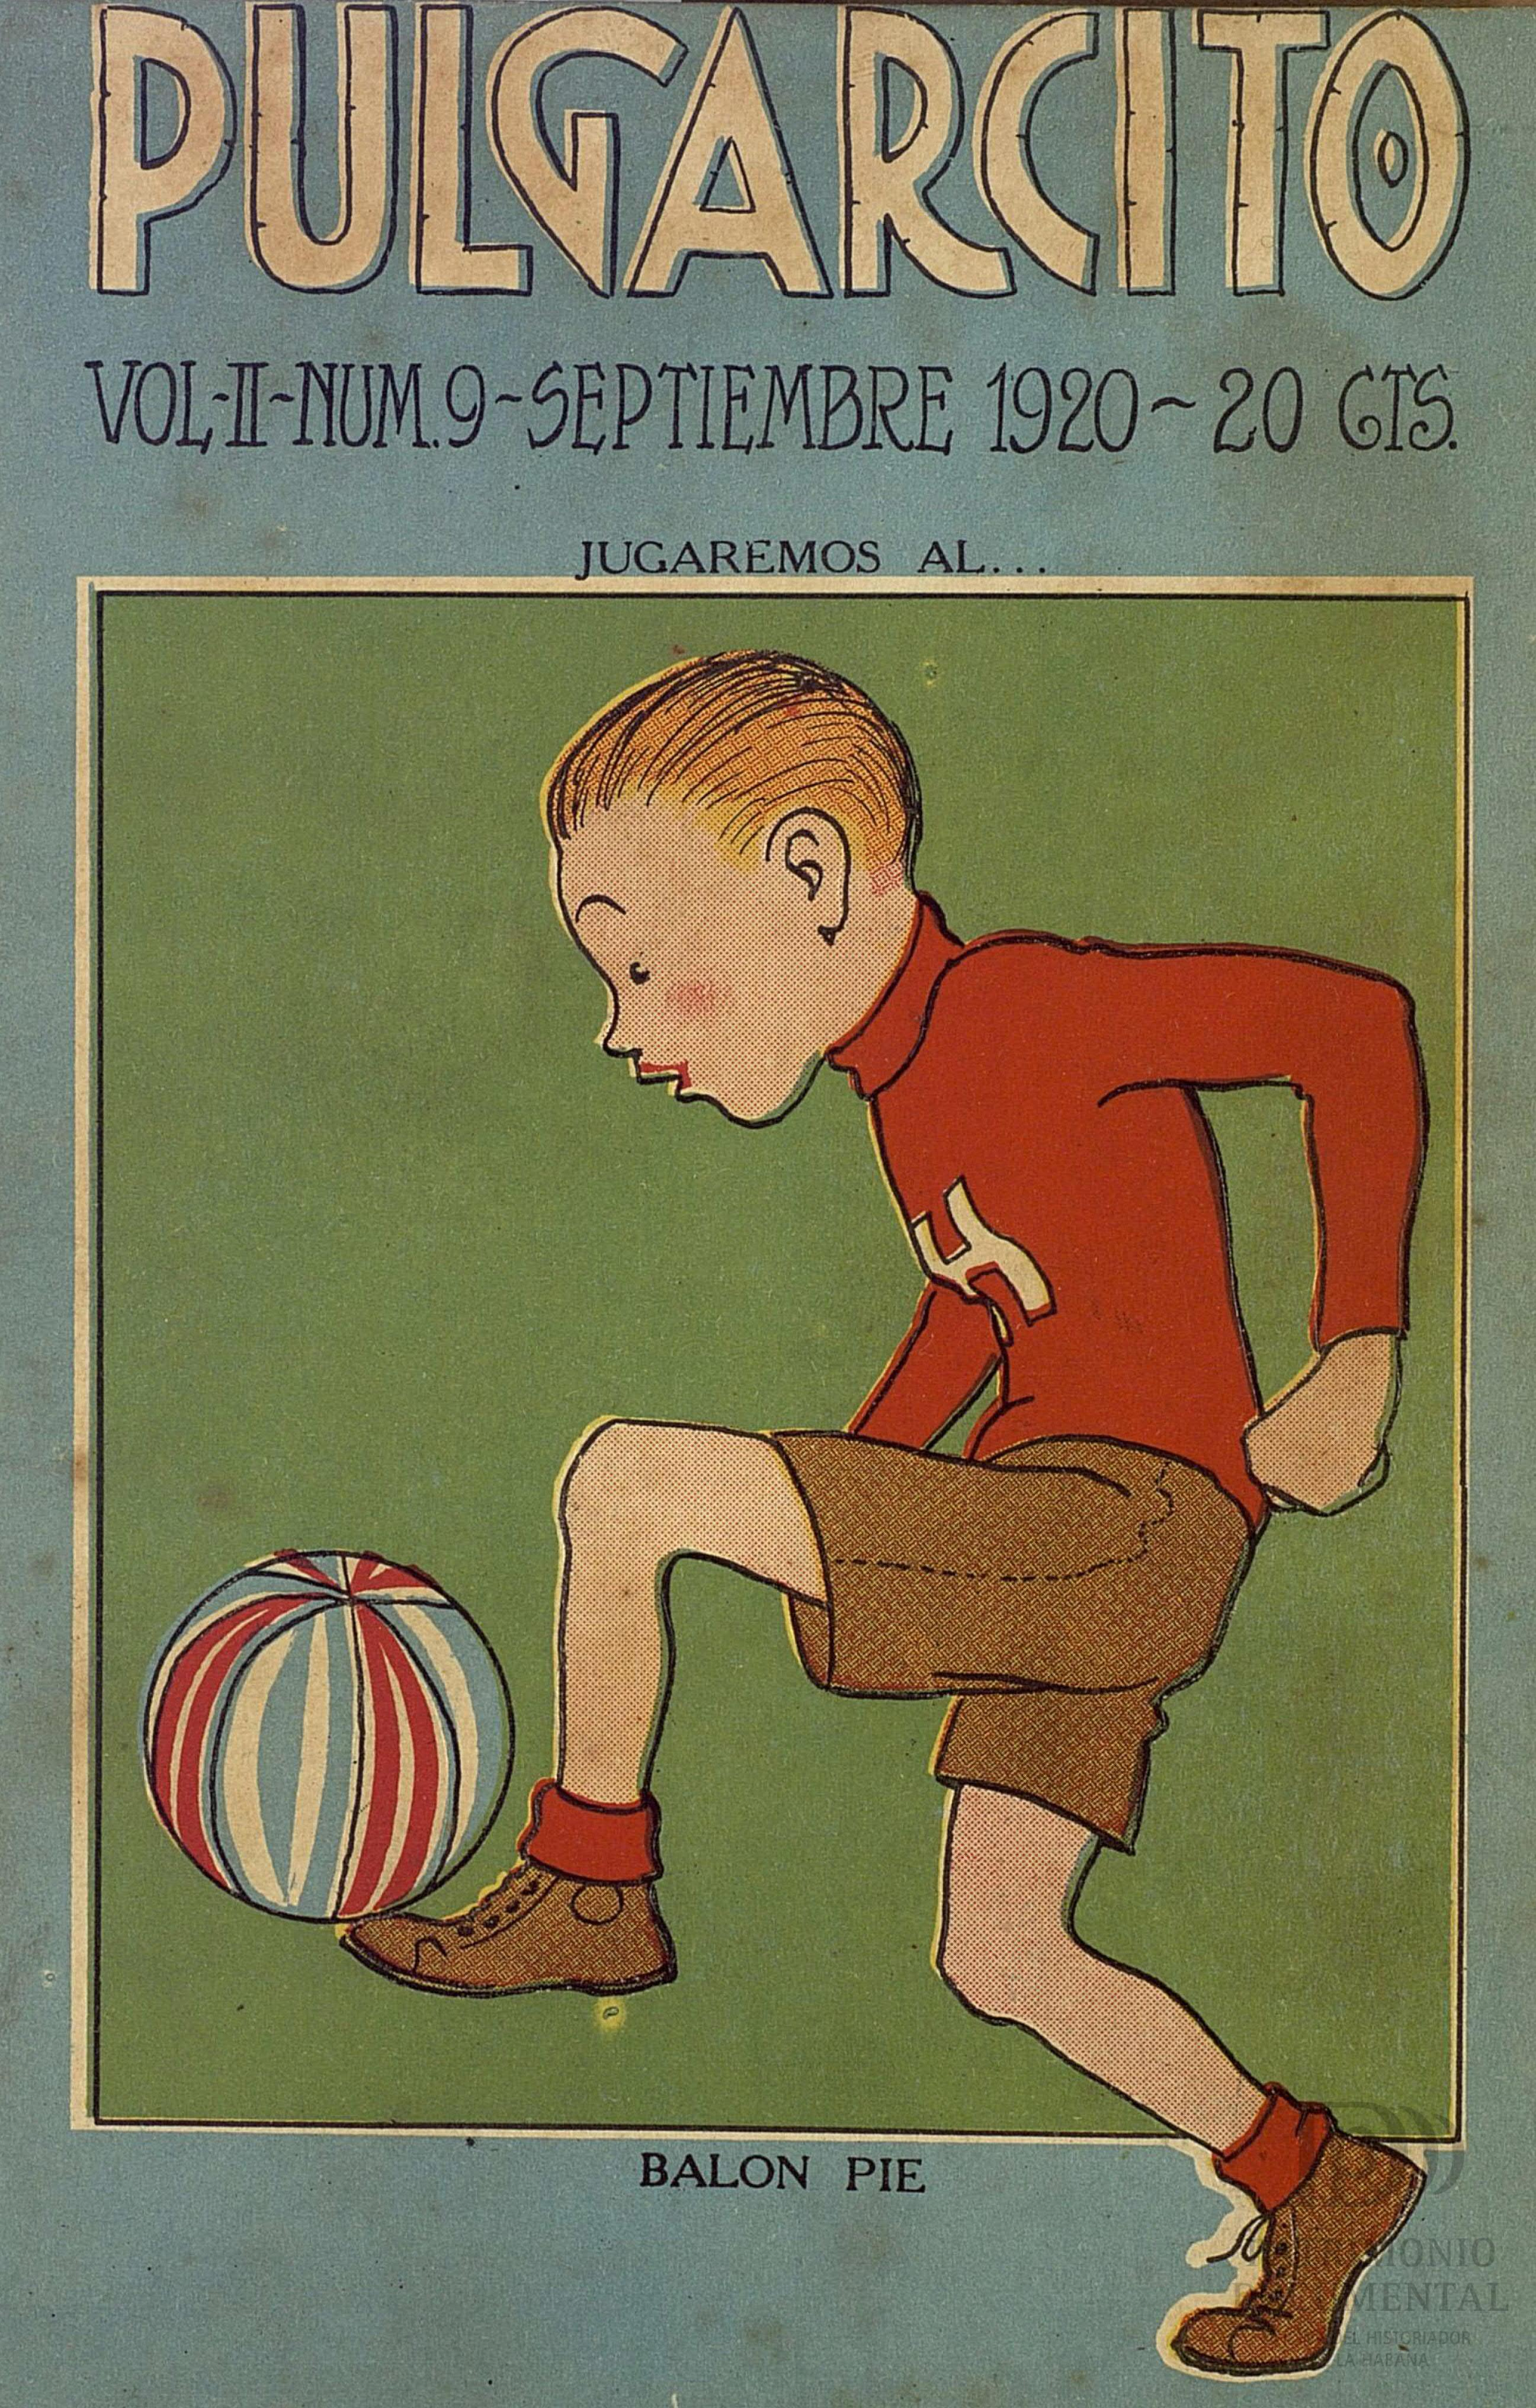
\includegraphics[width=0.5\textwidth]{Graphics/una portada de un libro con un ninho jugando con una pelota.jpg}
    \caption{Una portada de un libro con un niño jugando con una pelota (Exitoso)}
\end{figure}


\begin{figure}[h]
    \centering
    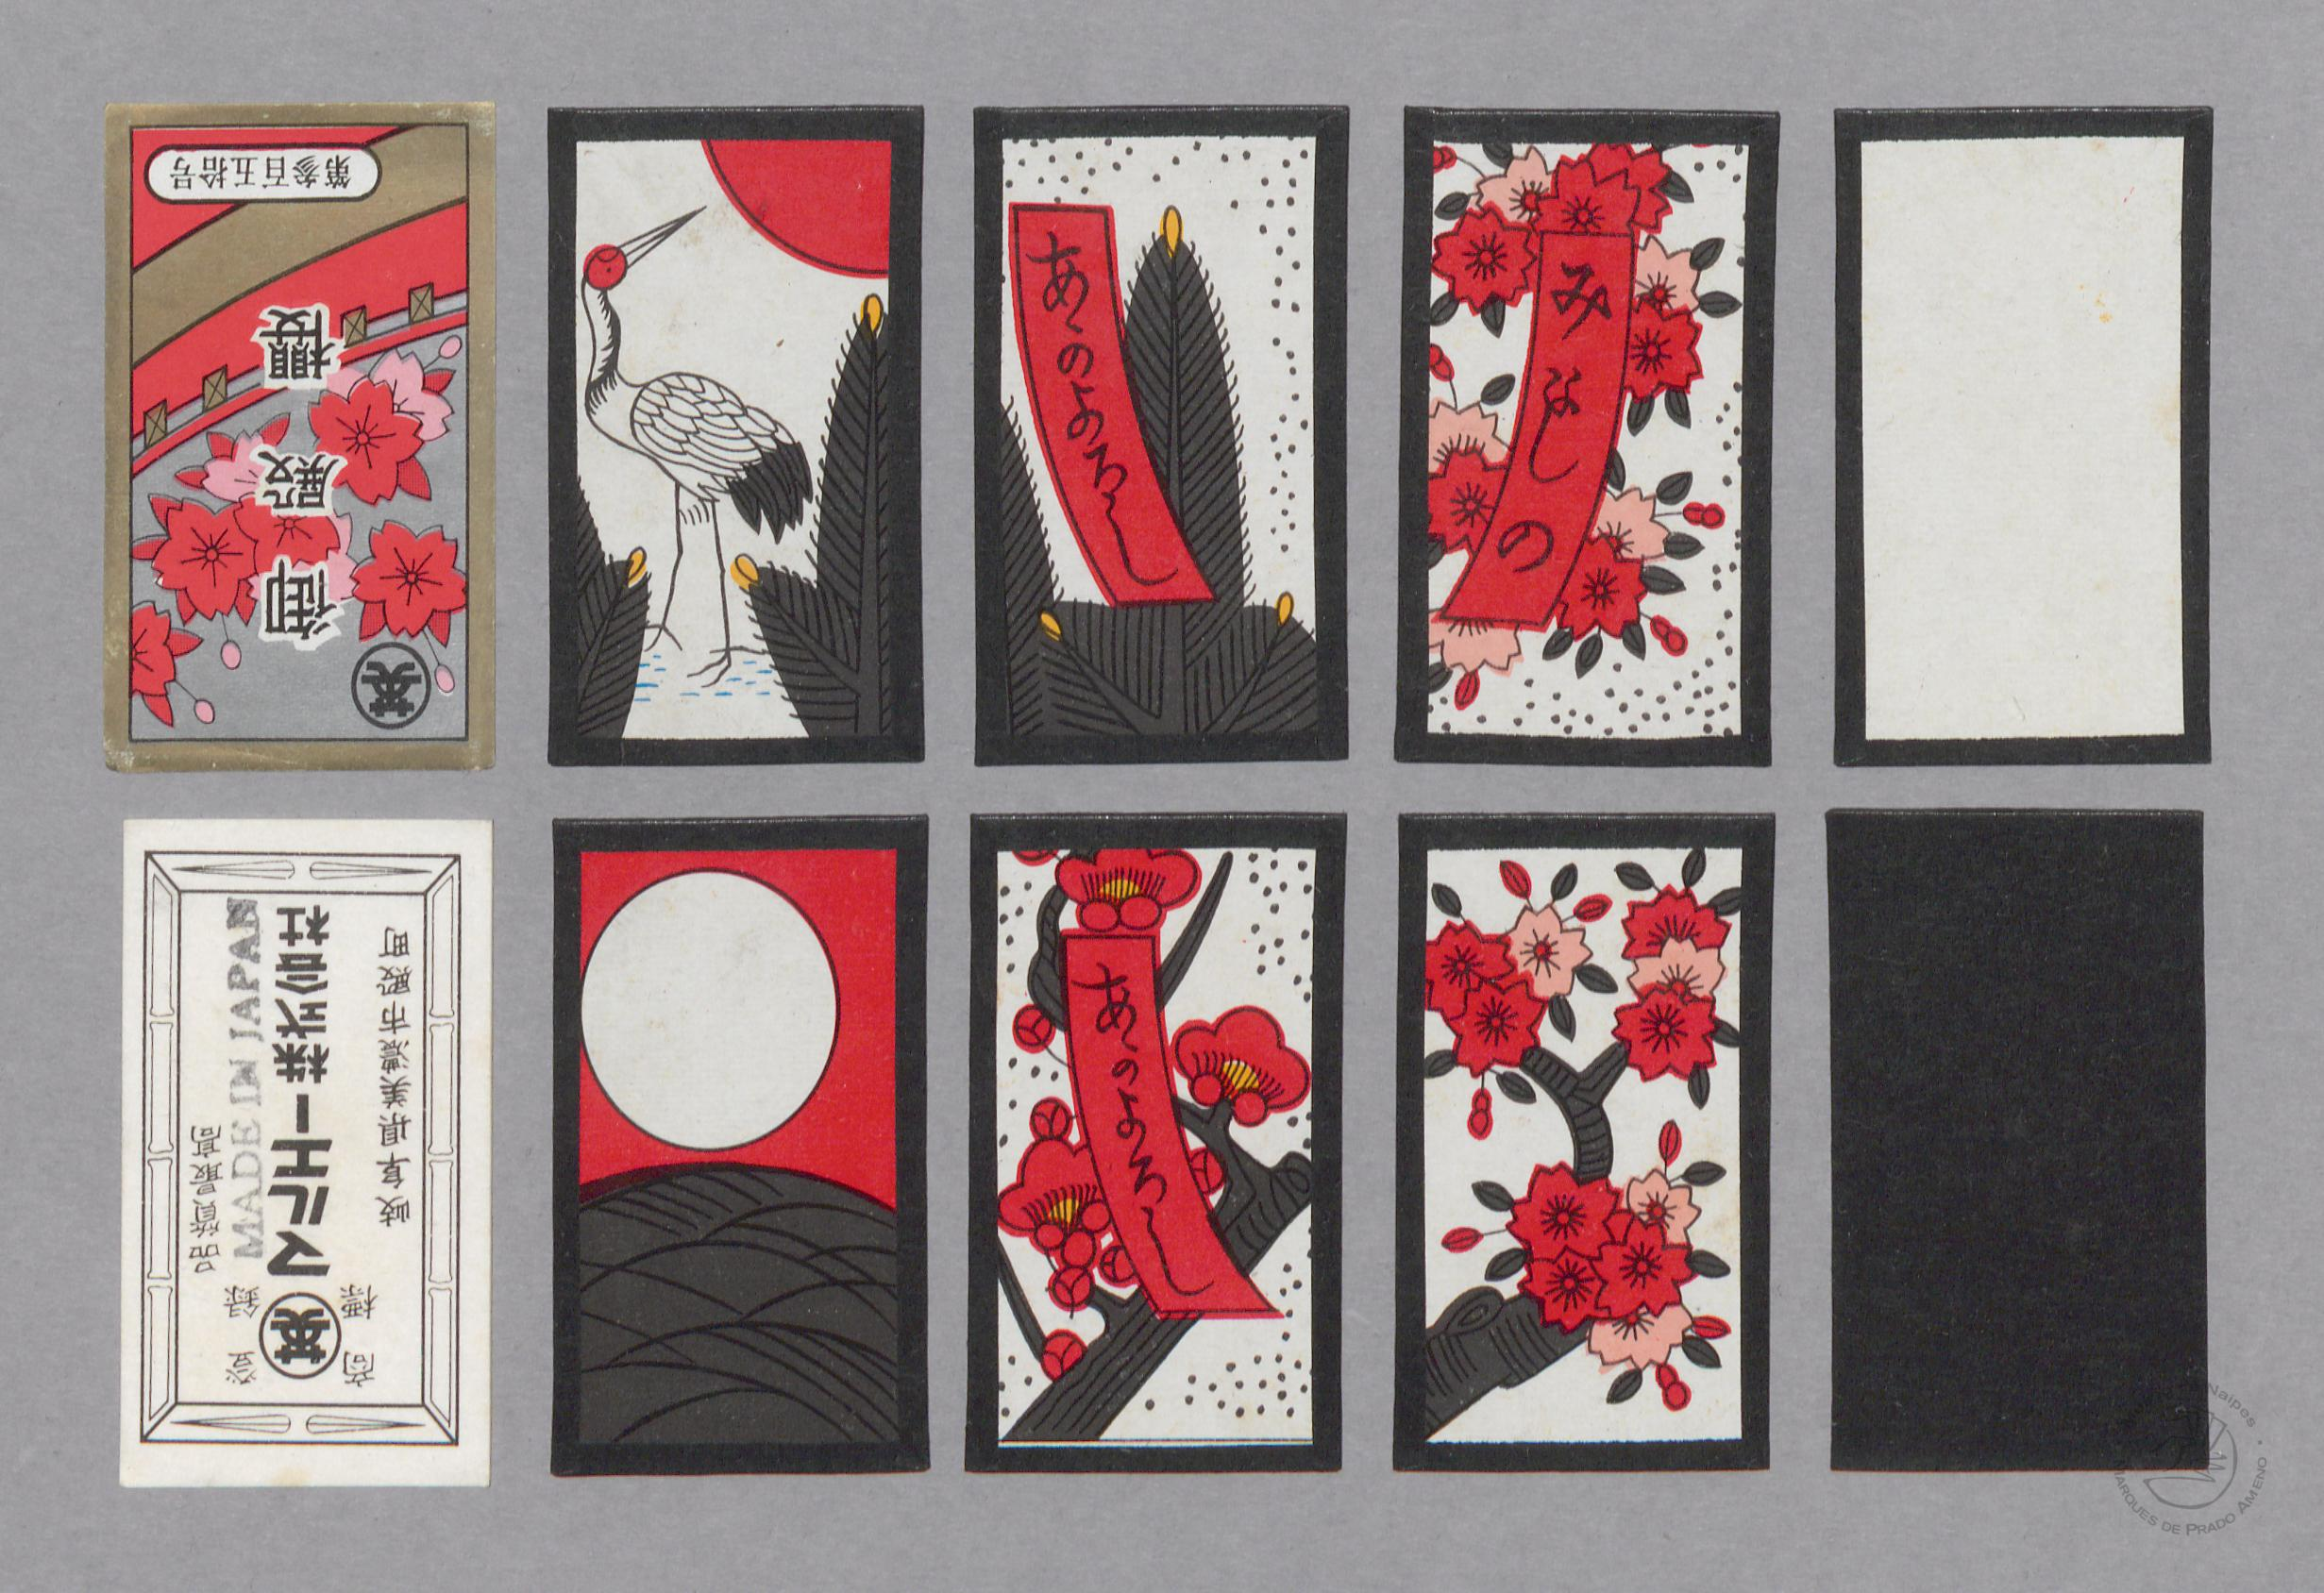
\includegraphics[width=0.5\textwidth]{Graphics/un grupo de seis japonenes jugando a las cartas.jpg}
        \caption{Un grupo de seis japonenes jugando a las cartas (Poco exitoso)}
    \end{figure}
    
    \begin{figure}[h]
        \centering
        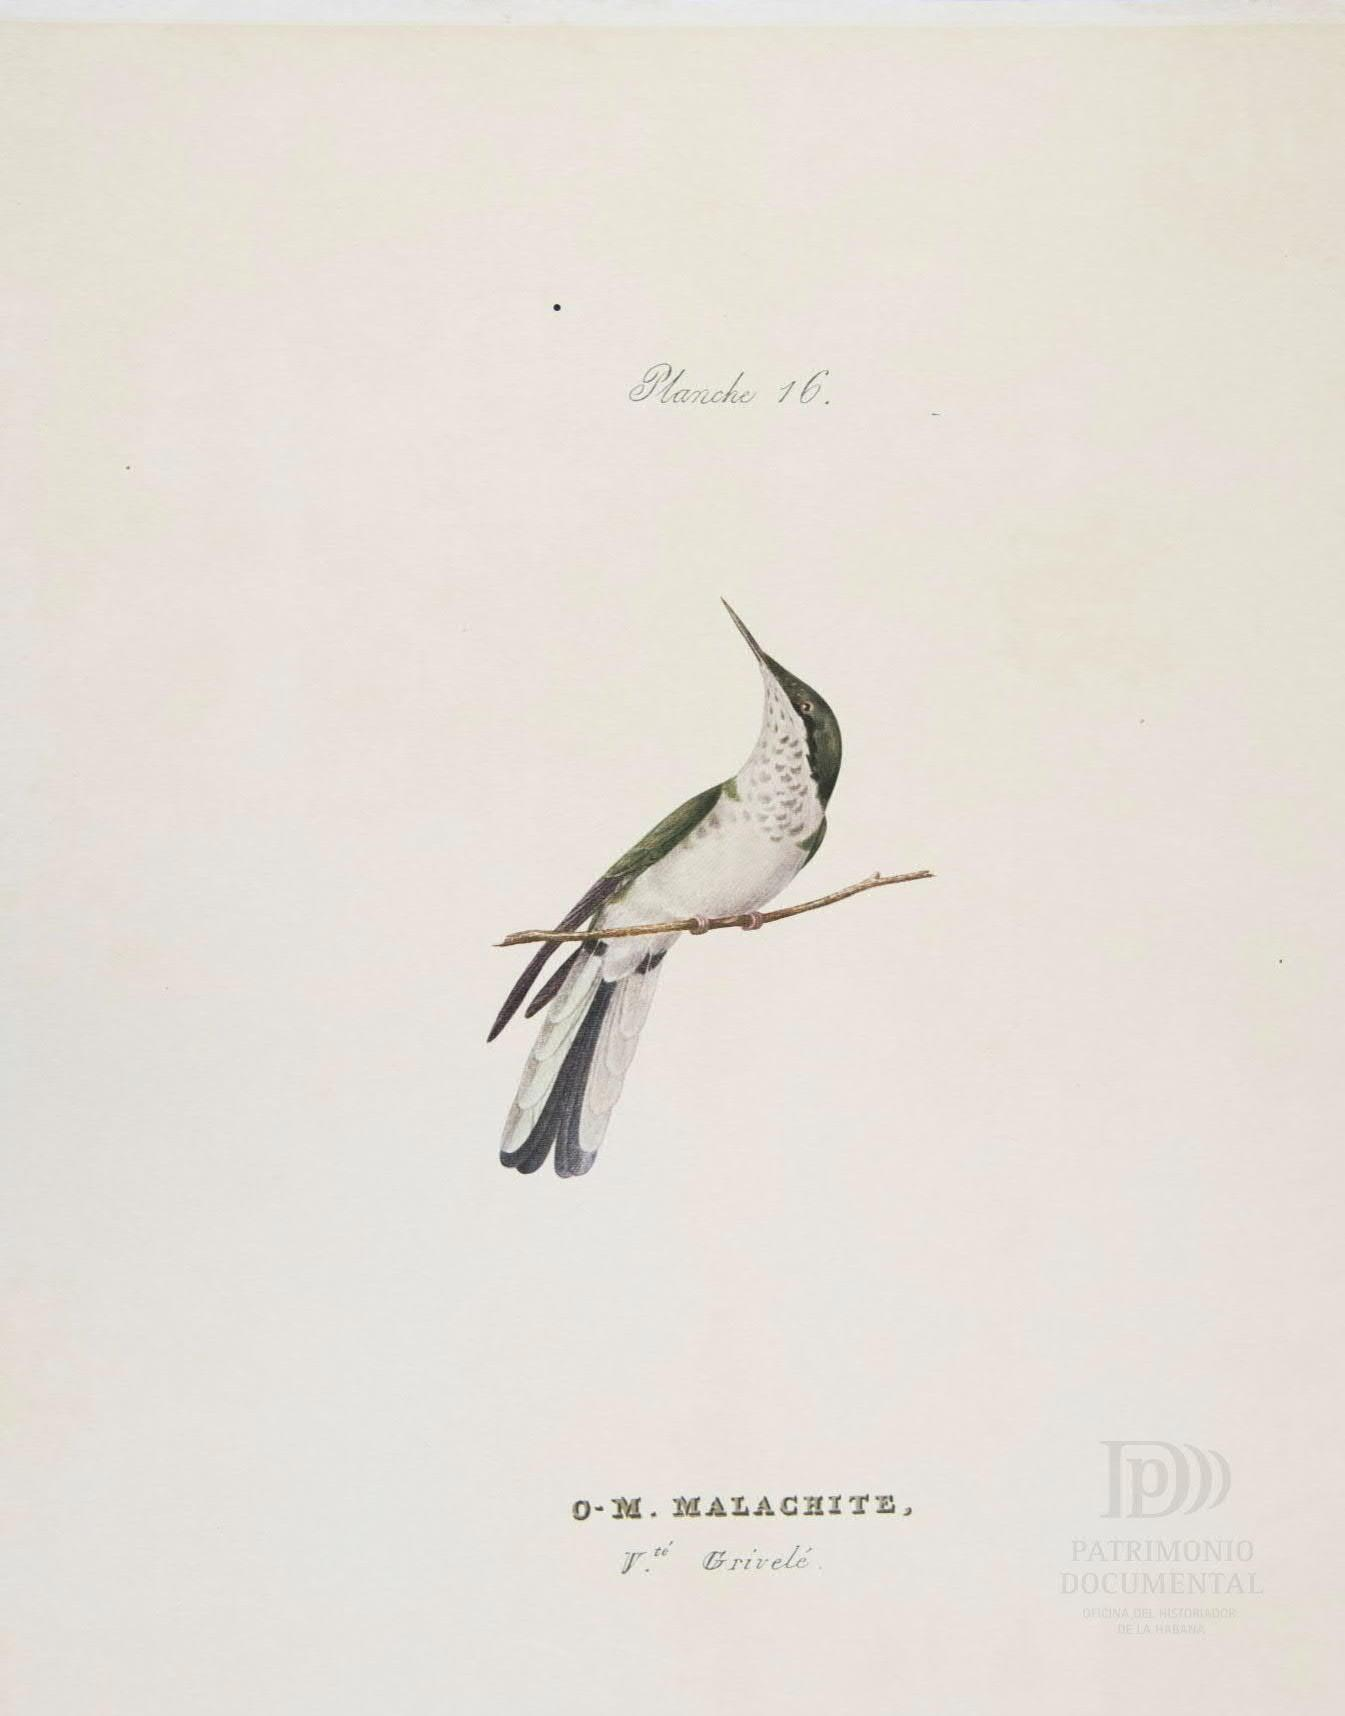
\includegraphics[width=0.5\textwidth]{Graphics/un pajaro sentado sobre una rama con las alas extendidas.jpg}
        \caption{Un pájaro sentado sobre una rama con las alas extendidas (Poco exitoso)}
    \end{figure}
    \begin{figure}[h]
        \centering
        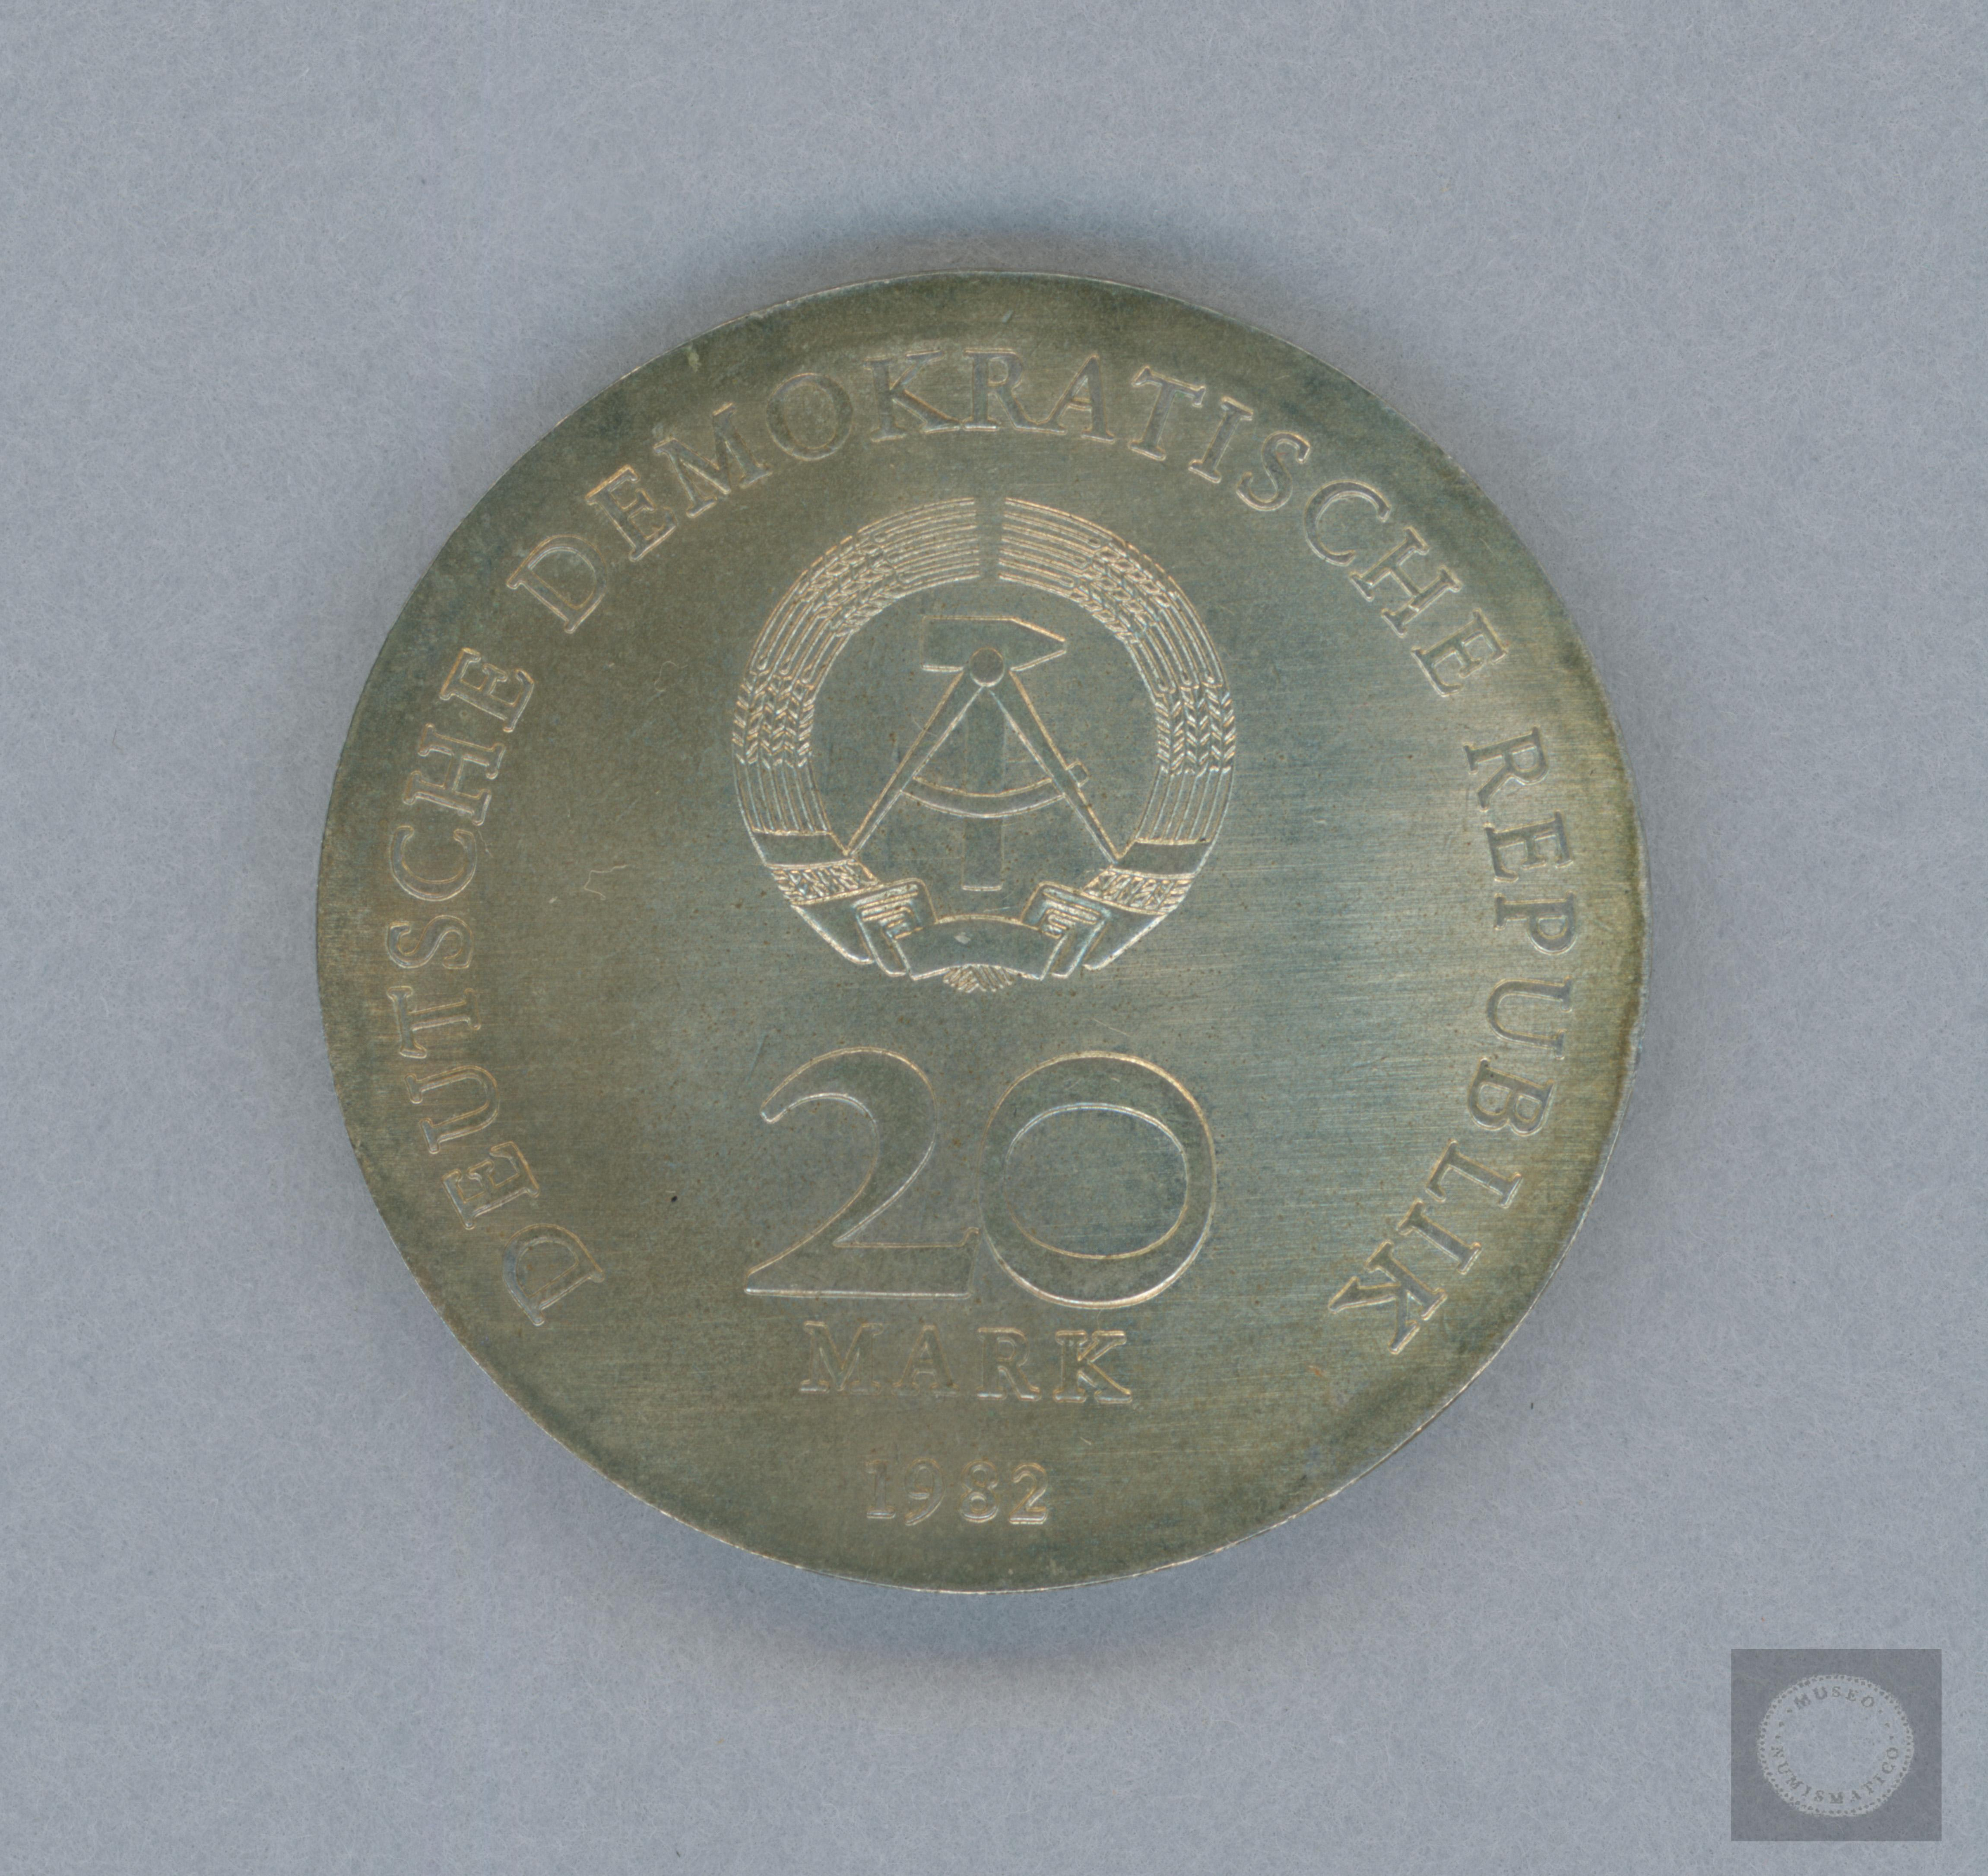
\includegraphics[width=0.5\textwidth]{Graphics/una moneda con una foto de un hombre en ella.jpg}
        \caption{Una moneda con una foto de un hombre en ella (Poco exitoso)}
\end{figure}


\begin{figure}[h!]
    \centering
    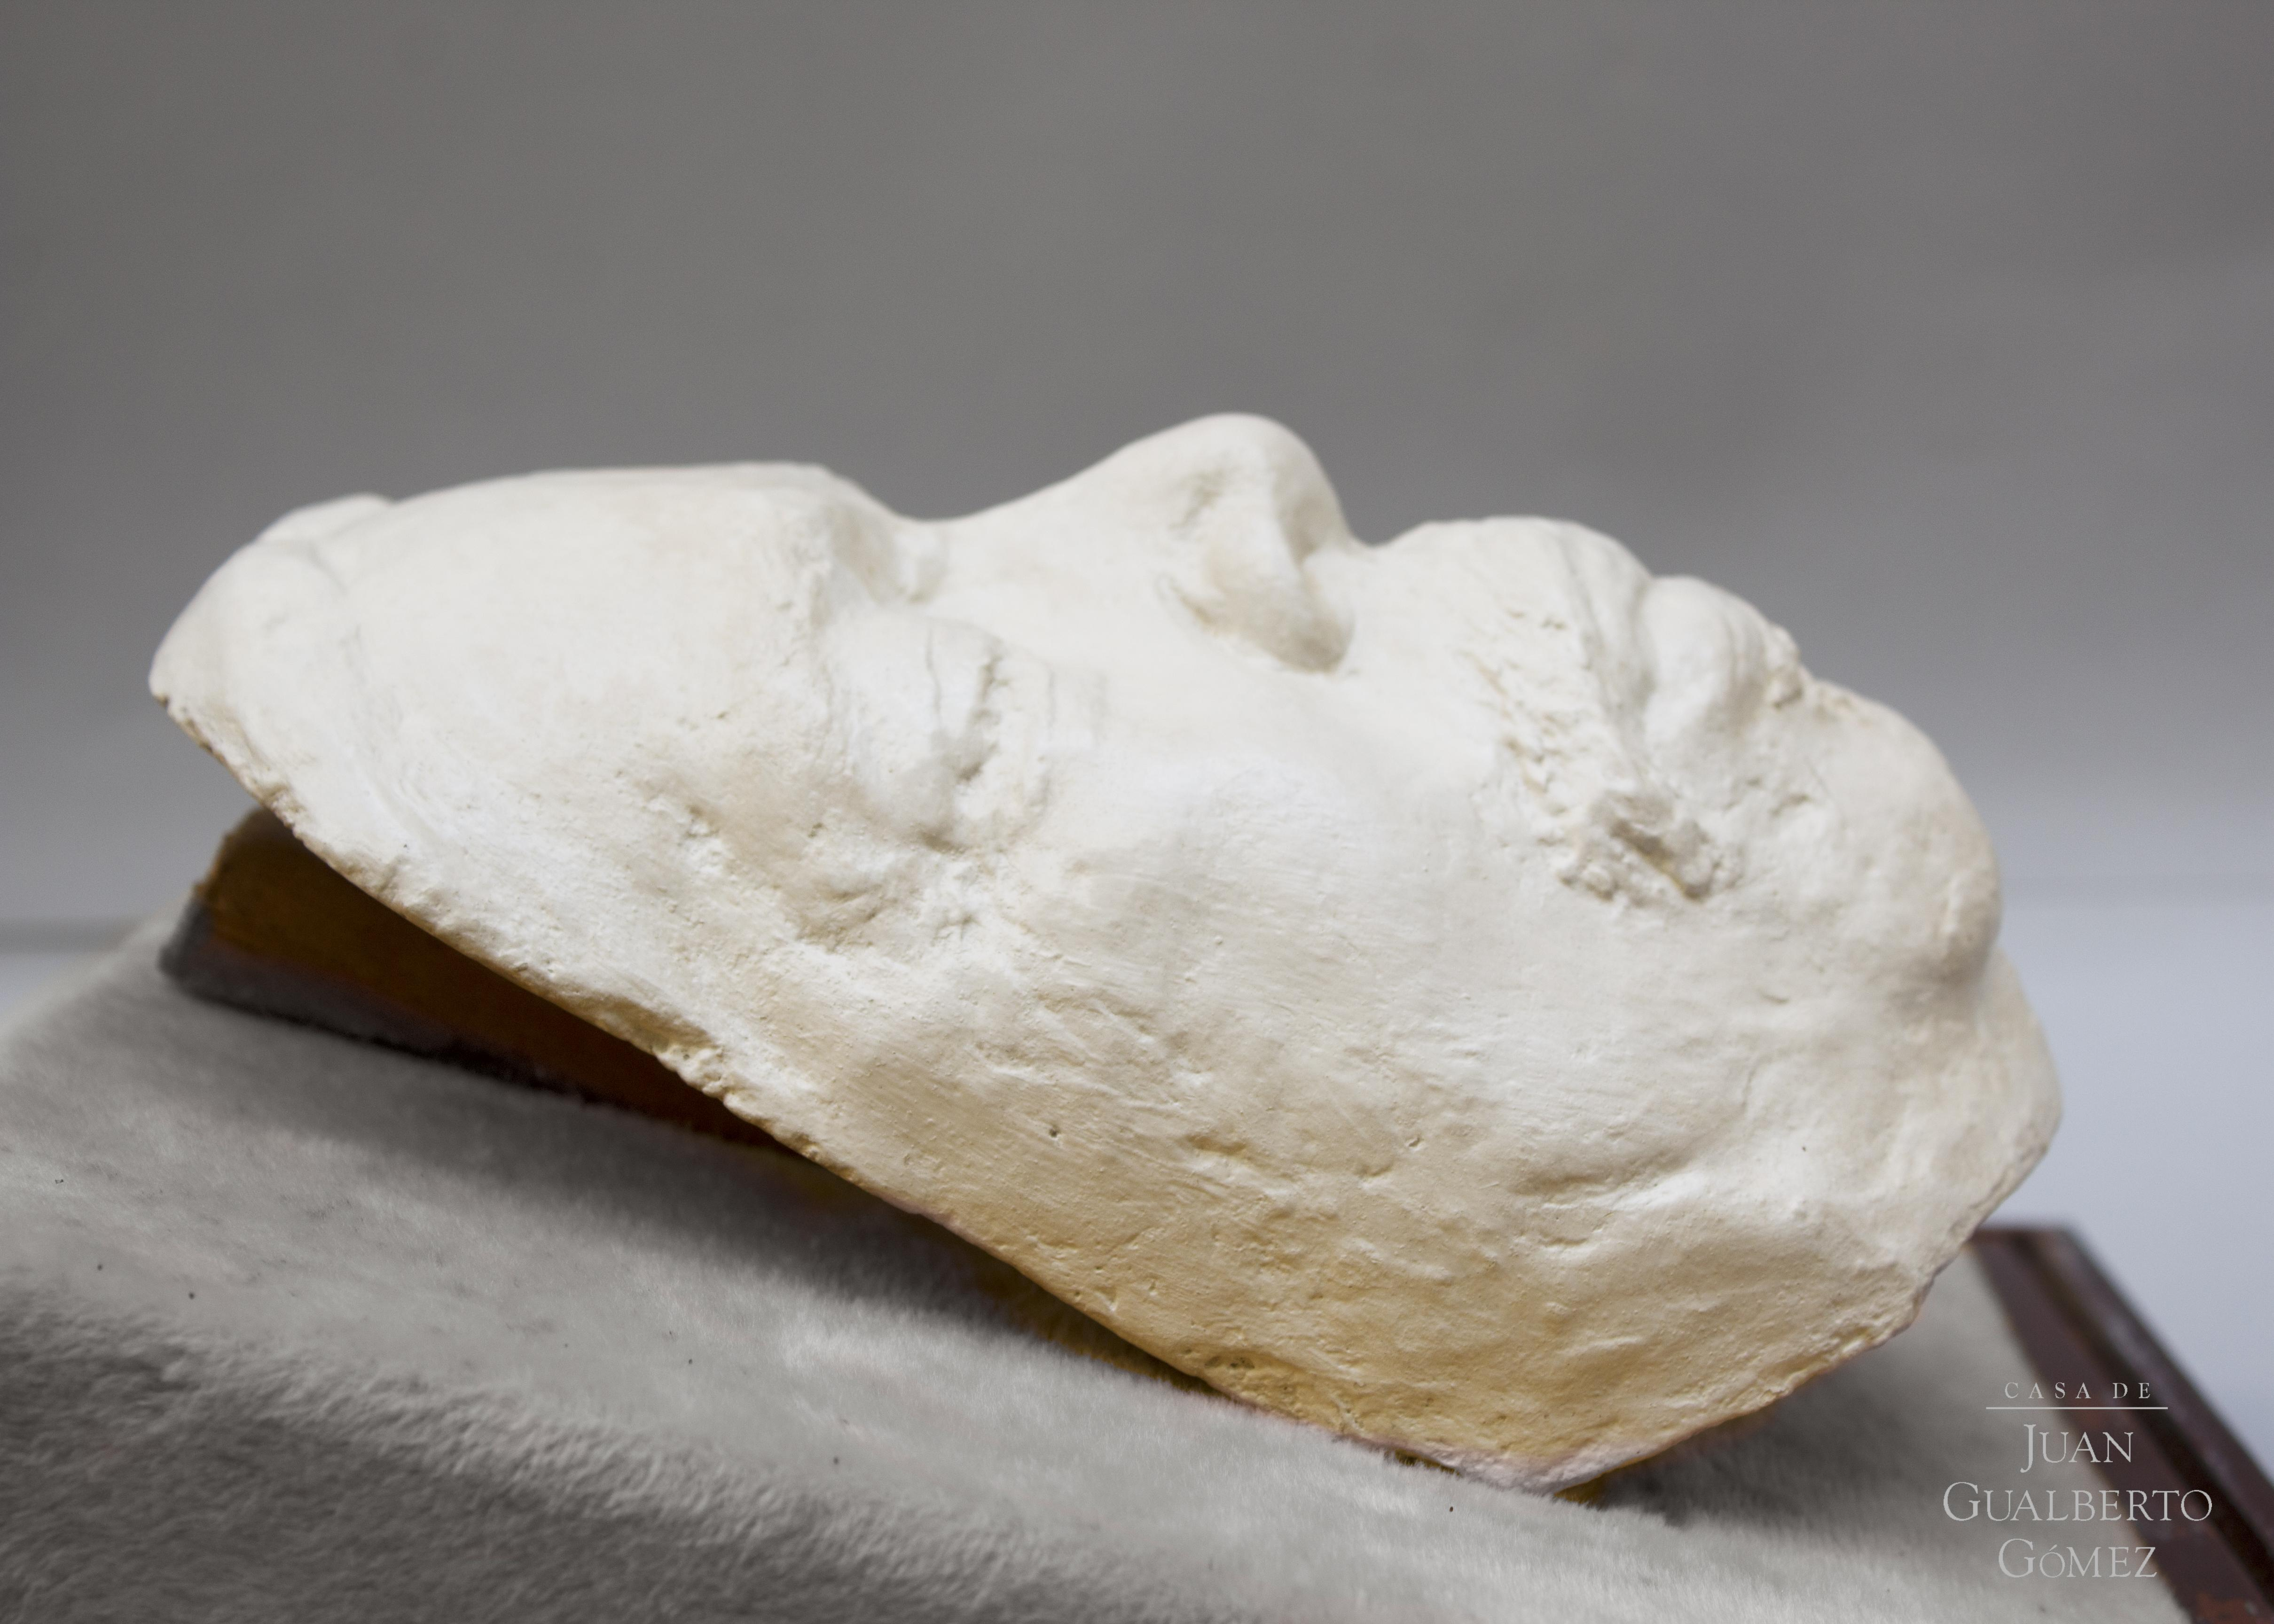
\includegraphics[width=0.5\textwidth]{Graphics/un pan blanco con un glaseado blanco.jpg}
        \caption{Un pan blanco con un glaseado blanco (No exitoso)}
    \end{figure}
    \begin{figure}[h!]
        \centering
        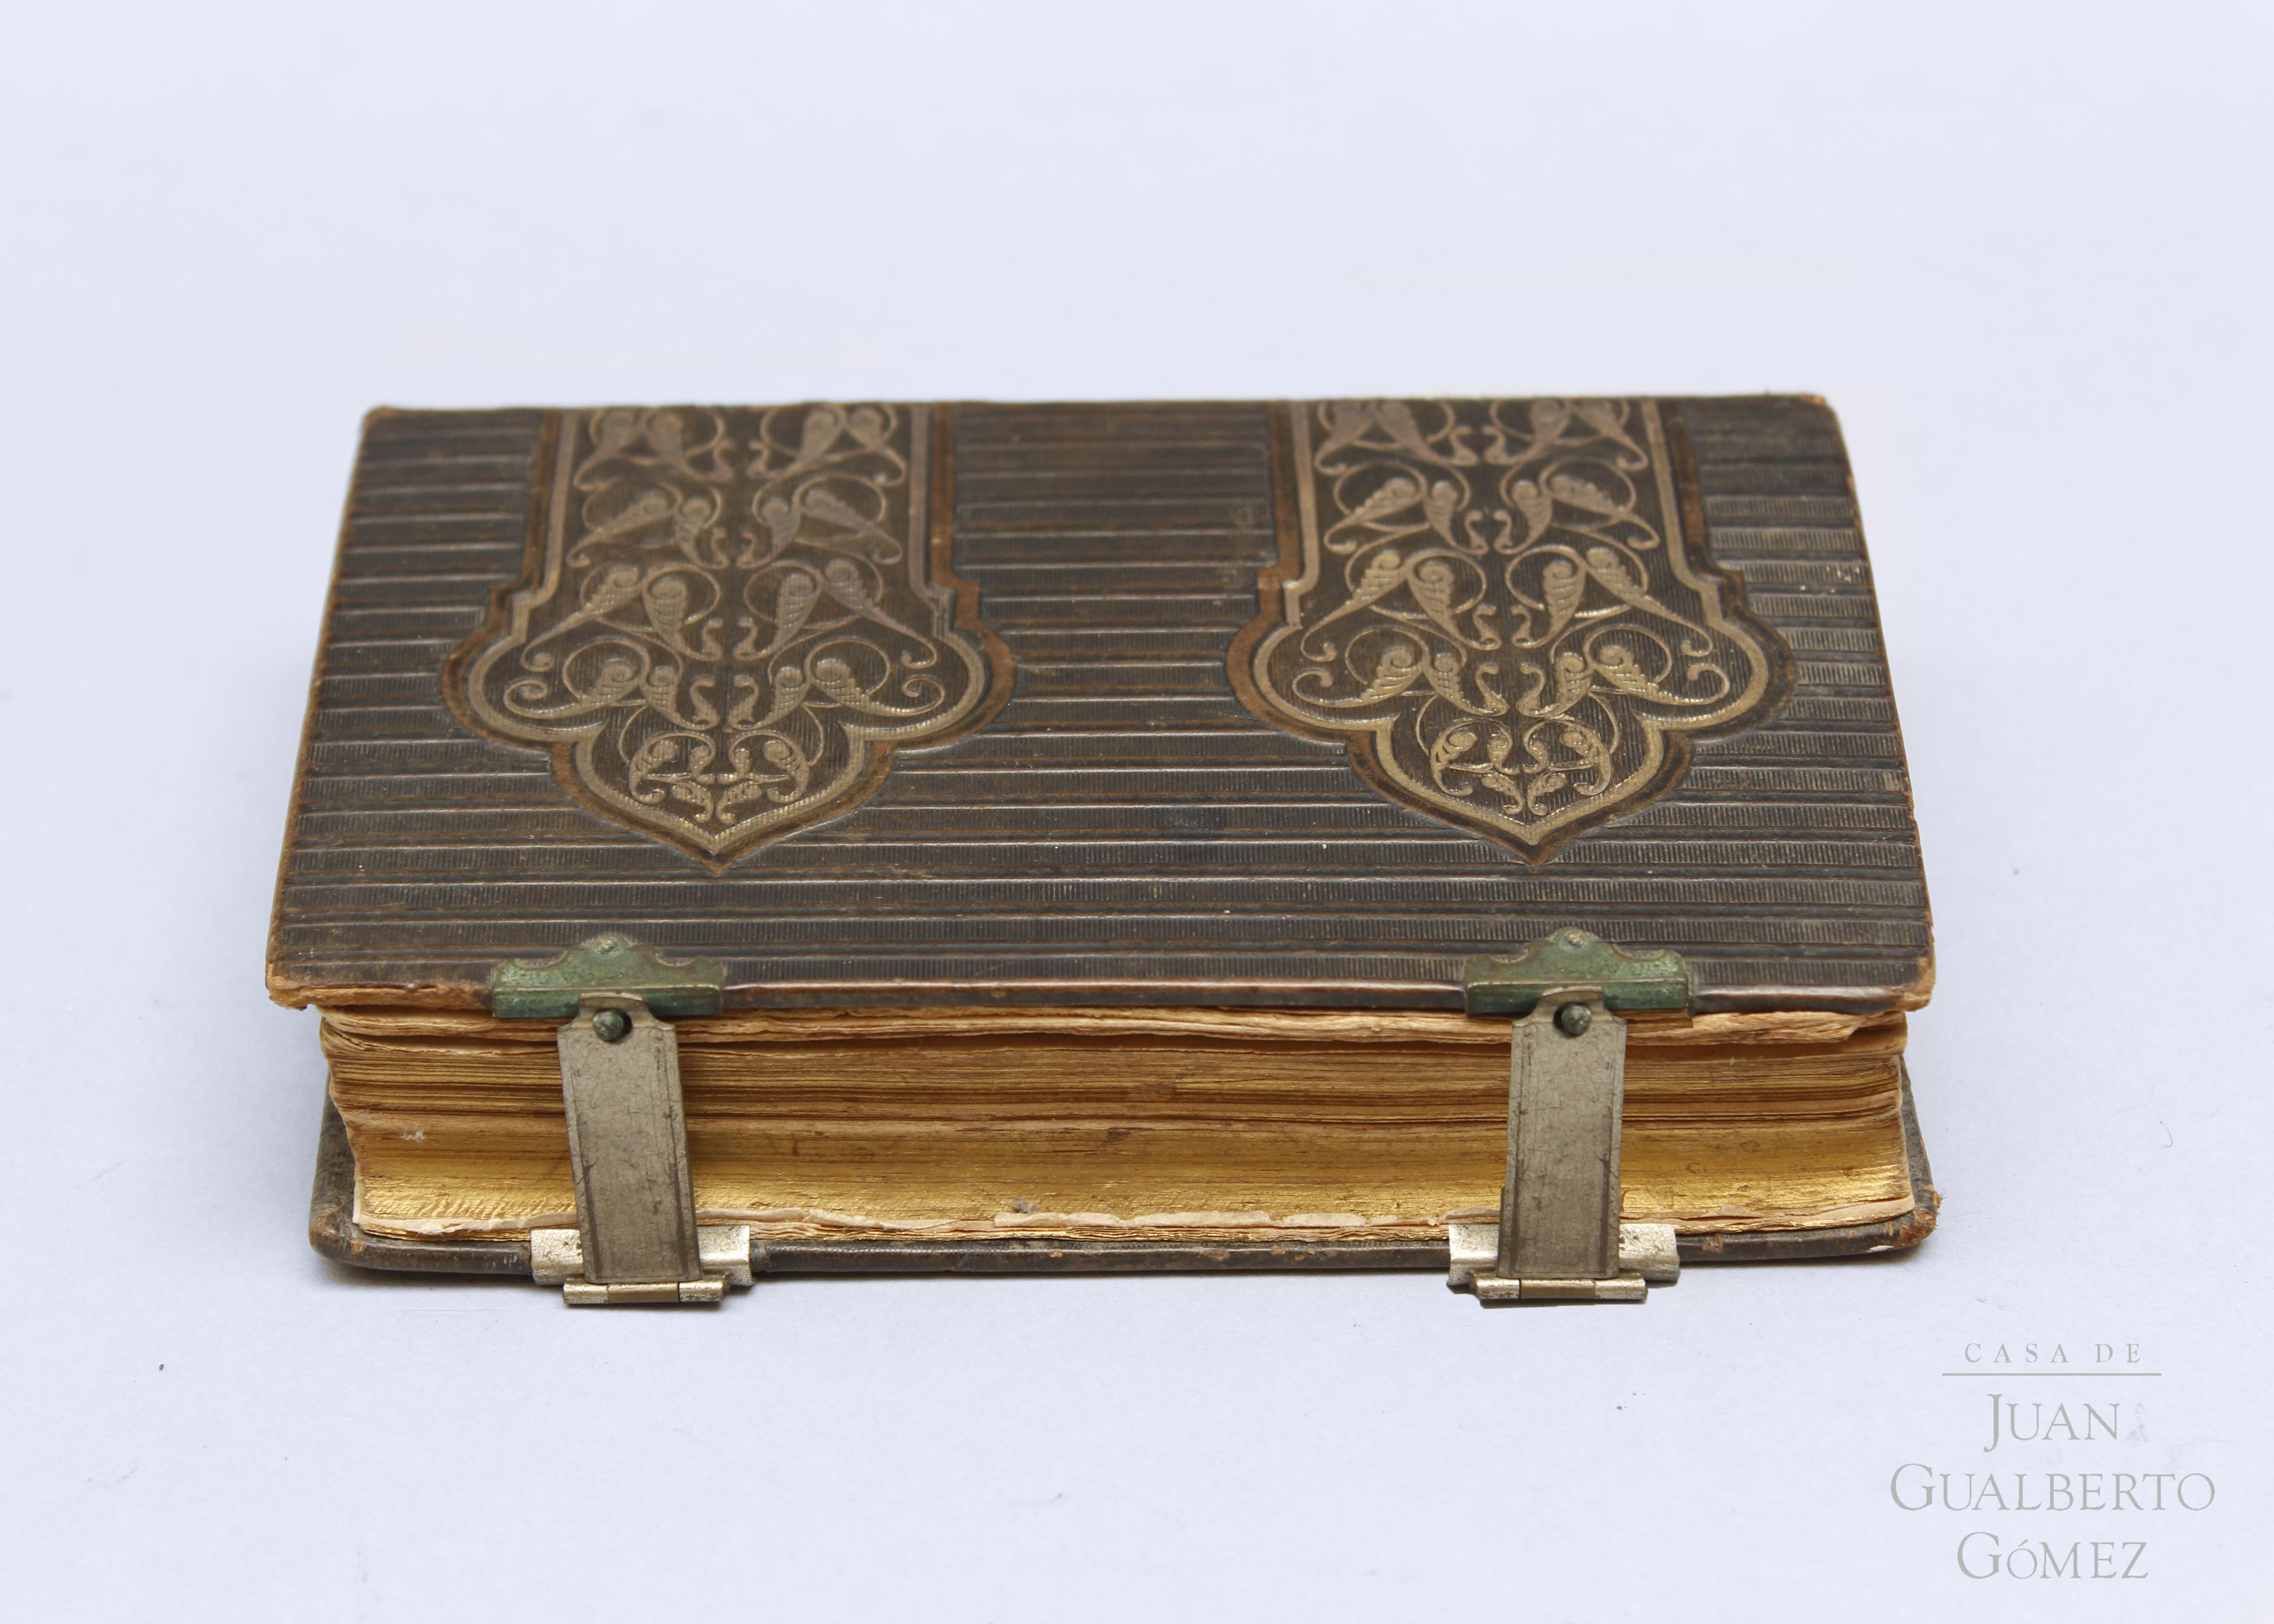
\includegraphics[width=0.5\textwidth]{Graphics/una caja pequenha con un mango de metal y un mango de metal.jpg}
        \caption{Una caja pequeña con un mango de metal y un mango de metal (No exitoso)}
    \end{figure}
    \begin{figure}[h!]
        \centering
        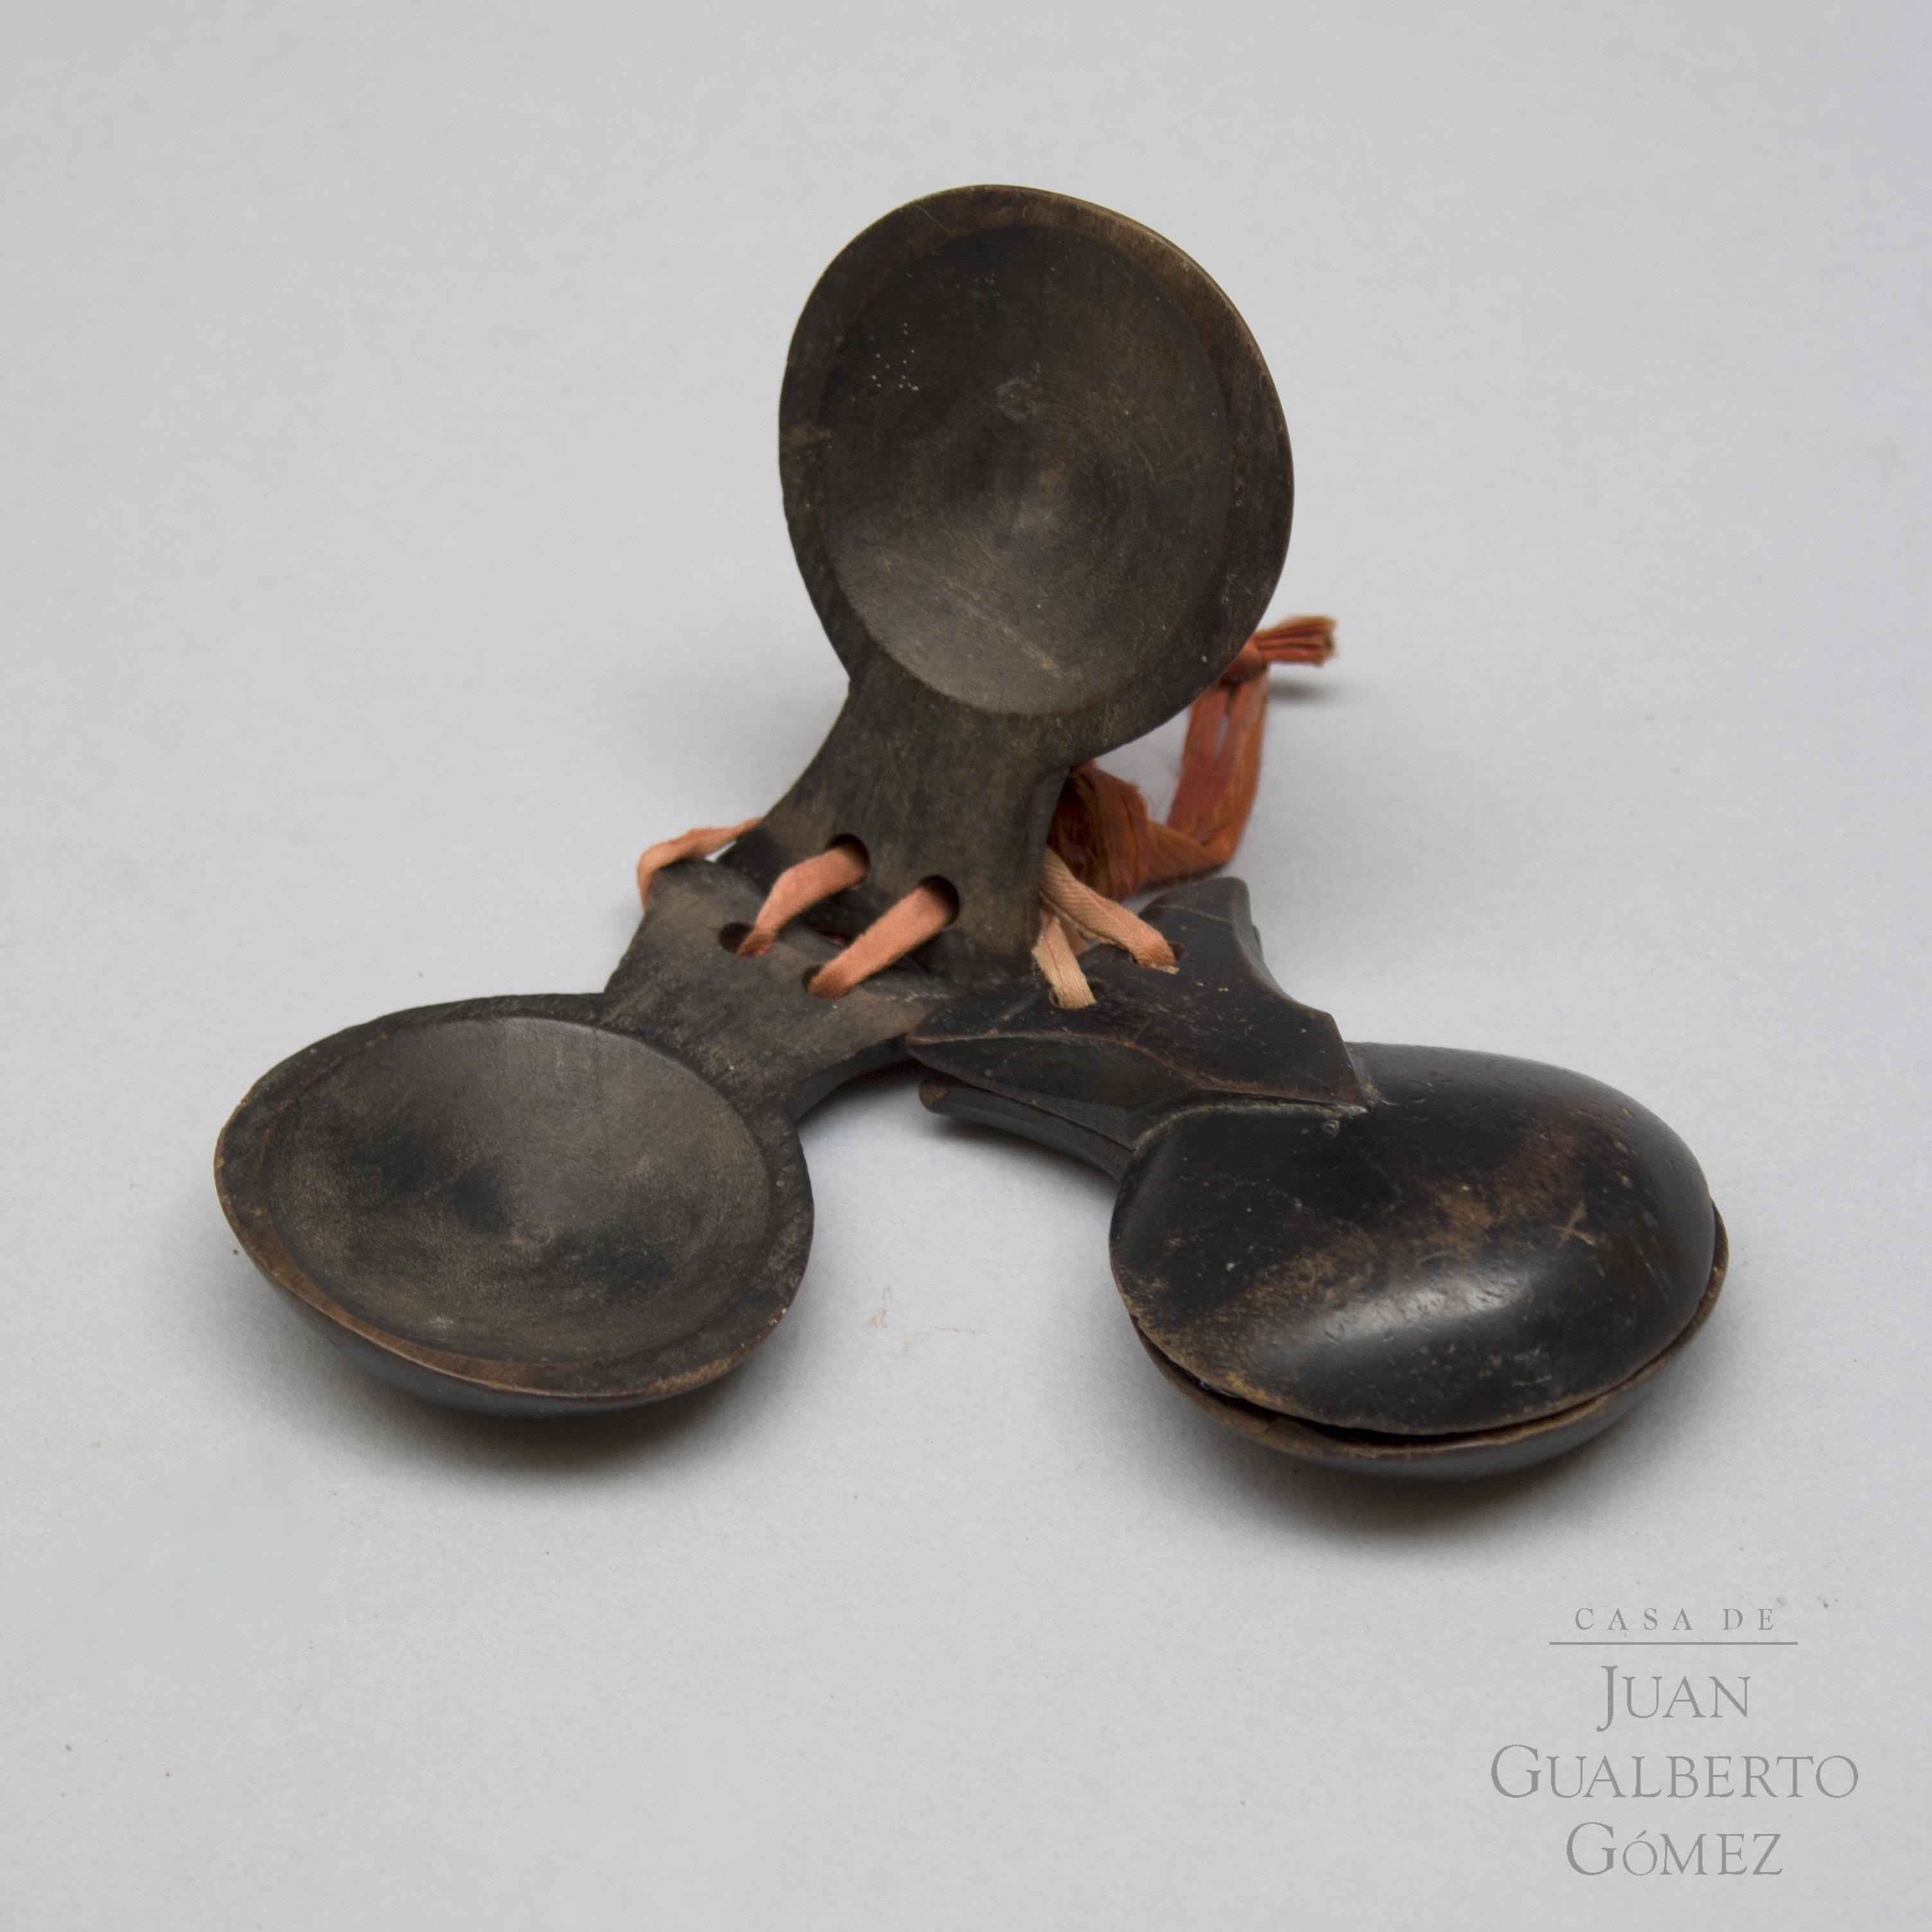
\includegraphics[width=0.5\textwidth]{Graphics/un juguete pequenho con un par de zapatos en el.jpg}
        \caption{Un juguete pequeño con un par de zapatos en él }
\end{figure}